%=====================================================
%====== If you are new to LaTeX, this website ========
%======     will be your new best friend:     ========
%======   http://en.wikibooks.org/wiki/LaTeX  ========
%======   Template created by Jonathan Blair  ========
%=====================================================



%=====================================================
%============ Controls ===============================
%=====================================================

%\documentclass[12pt,letterpaper,onecolumn]{article}
\documentclass[11pt,letterpaper,onecolumn]{article}
%\documentclass[10pt,letterpaper,onecolumn]{article}  % not recommended
%\documentclass[12pt,letterpaper,twocolumn]{article}
%\documentclass[11pt,letterpaper,twocolumn]{article}
%\documentclass[10pt,letterpaper,twocolumn]{article}


\usepackage{amsmath}
\usepackage{graphicx}
\usepackage{url}
\usepackage{textgreek}
\usepackage{float}
\usepackage{booktabs}
%\graphicspath{{path-to-folder-containing-necessary-graphics}{other folder as necessary}}


%=====================================================
%============ \begin{document} =======================
%=====================================================

\begin{document}

%=====================================================
%============ Title ==================================
%=====================================================

\title{\bf Observation of the Behavior of a NAND Logic Gate}
%\title{\Large\bf Larger, Bolded Title}

%=====================================================
%============ Author =================================
%=====================================================
\author{
 Jairo Portillo \\*
  \\*
 PHY 338K Electronic Techniques \\*
 Department of Physics \\*
 The University of Texas at Austin \\*
 Austin, TX 78712, USA
}
\date{April 21, 2016}

%\address{The University of Texas, Austin, Texas, 78712}

\maketitle

%=====================================================
%============ Abstract ===============================
%=====================================================

\begin{abstract}

In this lab, we will explore the behavior of a Logic Gates. We will confirm the expected truth table of the NAND Logic Gate and determine the truth table for a three input NAND. We will also observe and confirm the behavior of a contact bounce eliminator NAND.

\end{abstract}

%=====================================================
%============ Body of the article ==========================
%=====================================================

%=====================================================
%============ Section ==================================
%=====================================================

\section{Preperation}

 In order to prepare for this lab, we must go over the Boolean functionality of the logic gates specifically a NAND gate. For logic gates, 1 is TRUE and 0 is FALSE. 1 indicates there is an input voltage and 0 indicates there is no voltage. 
 
 \begin{table}[H]
\centering
\begin{tabular}{|c|c|c|}
 \hline
 A & B & F \\\hline
 0 & 0 & 0 \\
 0 & 1 & 0 \\
 1 & 0 & 0 \\
 1 & 1 & 1 \\
  \hline

\end{tabular}
\caption{AND Gate Behavior}
\label{tab:AND}
\end{table}

An AND Gate follows the the A and B Boolean function. As seen in Table 1, TRUE and TRUE gives TRUE while TRUE and FALSE returns FALSE.
 
 \begin{table}[H]
\centering
\begin{tabular}{|c|c|c|}
 \hline
 A & B & F \\\hline
 0 & 0 & 1 \\
 0 & 1 & 1 \\
 1 & 0 & 1 \\
 1 & 1 & 0 \\
  \hline

\end{tabular}
\caption{NAND Gate Behavior}
\label{tab:NAND}
\end{table}

On the other hand a NAND Gate follows the Boolean function
$$\text{Not(A and B)}$$
As seen in Table 2, NOT(TRUE and TRUE) gives FALSE while NOT(TRUE and FALSE) returns TRUE.

\subsection{Data Collection}




\section{Lab work}

\subsection{Apparatus}

This lab will use a DC power supply, a two NAND logic gate chip, two low resistors of the same resistance in our case 2.2 k$\Omega$, and led to confirm output.


\subsection{Data Collection}

For the first portion of the lab we simply confirmed the truth table of a singe NAND gate which we were able to.

\begin{table}[H]
\centering
\begin{tabular}{|c|c|c|}
 \hline
 A & B & F \\\hline
 0 & 0 & 1 \\
 0 & 1 & 1 \\
 1 & 0 & 1 \\
 1 & 1 & 0 \\
  \hline

\end{tabular}
\caption{NAND Gate Results}
\label{tab:data}
\end{table}

For the second portion, we found the truth table of a three input nand gate. This can bee seen in Figure 1 below, the output of one NAND gate goes into one of the inputs of another NAND gate.  

\begin{figure}[H]
    \centering
    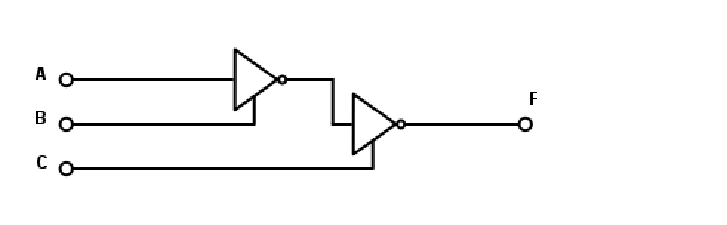
\includegraphics{Triput.pdf}
    \caption{Our common emitter amplifier circuit. With node as the AC input and a DC voltage input}
    \label{fig:my_label}
\end{figure} 
A three input NAND gate yields a Boolean function of
$$\text{NOT( NOT( A and B) and C)}$$


\begin{table}[H]
\centering
\begin{tabular}{|c|c|c|c|}
 \hline
 A & B & C & F \\\hline
 0 & 0 & 0 & 1\\
 1 & 0 & 0 & 1\\
 1 & 1 & 1 & 1\\
 0 & 1 & 1 & 1\\
 0 & 0 & 1 & 1\\
 0 & 1 & 0 & 1\\
 1 & 0 & 1 & 0\\
 
  \hline

\end{tabular}
\caption{Three input NAND Gate Results}
\label{tab:data1}
\end{table}

Finally we tested the contact bounce eliminator switch and how the output will only change once when the switch is contacted multiple times.

\begin{figure}[H]
    \centering
    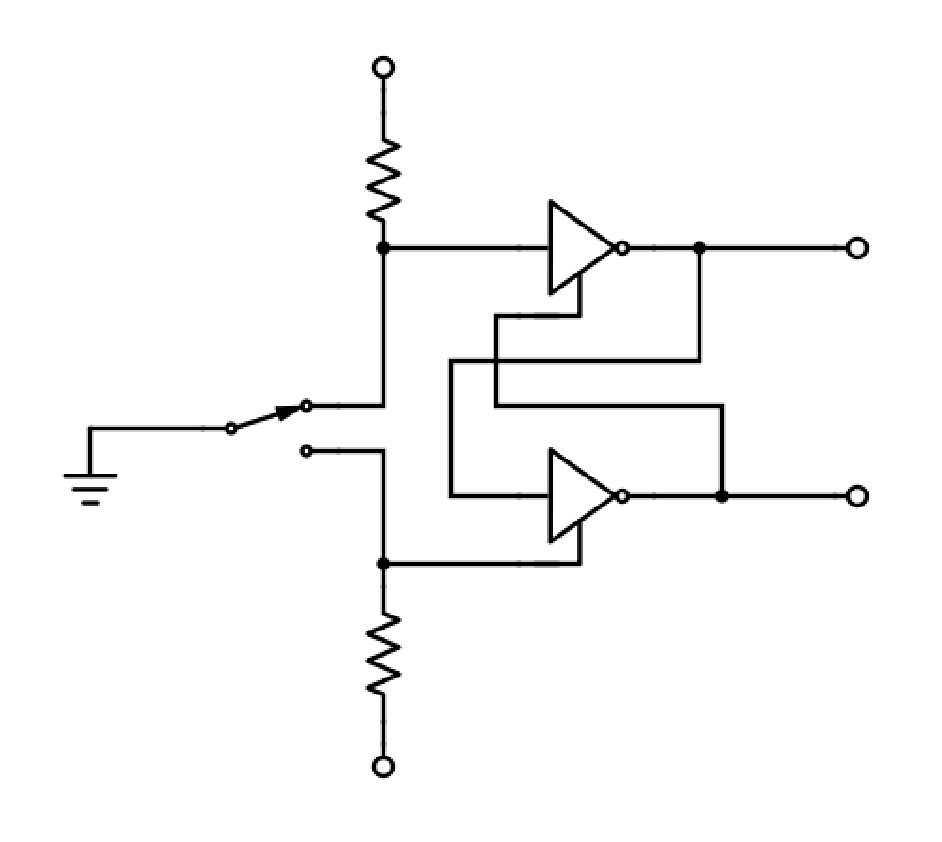
\includegraphics[scale = .75]{cross1.pdf}
    \caption{A Contact Bounce Eliminator NAND with 2.2 k$\Omega$ resistors.}
    \label{fig:data2}
\end{figure} 

For our actual circuit there was no switch but simply moving where the ground connected to in place of the switch. We were able to confirm that the output only changes once when the respective terminal is contacted with ground. 

\section{Summary and conclusions}

In this lab we observed how NAND logic gate follows the behavior of the Boolean function
$$\text{Not(A and B)}$$
and the three input NAND follows the 
$$\text{NOT( NOT( A and B) and C)}$$
Boolean function. We were able record these behavior and confirm the switch behavior of the contact bounce eliminator. 





%=====================================================
%============ Bibliography  ==============================
%=====================================================



%=====================================================
%============ End ====================================
%=====================================================

\end{document}

%=====================================================
%============ End ====================================
%=====================================================